\documentclass[a4paper,10pt,titlepage]{article}

\usepackage{geometry}
\usepackage{amsmath}
\usepackage{amssymb}
\usepackage{txfonts}
\usepackage{microtype}
\usepackage{epsfig}
\usepackage{graphicx}
\usepackage{moreverb}
\usepackage{hyperref}
\usepackage{listings}
\usepackage{xcolor}
\usepackage{textcomp}
\definecolor{listinggray}{gray}{0.98}
\definecolor{lbcolor}{rgb}{0.98,0.98,0.98}
\lstset{
	backgroundcolor=\color{lbcolor},
	tabsize=4,
	rulecolor=,
	language=matlab,
    basicstyle=\scriptsize\ttfamily,
    upquote=true,
    aboveskip={1.5\baselineskip},
    columns=fixed,
    showstringspaces=false,
    extendedchars=true,
    breaklines=true,
    prebreak = \raisebox{0ex}[0ex][0ex]{\ensuremath{\hookleftarrow}},
    frame=single,
    showtabs=false,
    showspaces=false,
    showstringspaces=false,
    identifierstyle=\ttfamily,
    keywordstyle=\color[rgb]{0,0,1},
    commentstyle=\color[rgb]{0.133,0.545,0.133},
    stringstyle=\color[rgb]{0.627,0.126,0.941},
}
\usepackage{eso-pic}
\usepackage{ifthen}

\AddToShipoutPictureBG{\ifthenelse{\equal{\value{page}}{0}}{}{
\includegraphics{template_files/backgroundlines}}}


\usepackage{tikz}
\usepackage{pgfplots}
\usepackage{tikzscale}
\usepackage{graphicx}
\usepackage{float}
\usepackage{subcaption}
\usepackage{comment}
\usepackage{units}
\usetikzlibrary{external}\tikzexternalize


\title{H3b: Time dependent quantum mechanics}
\author{Victor Nilsson and Simon Nilsson (930128-1854)}
\date{\today}

\begin{document}

\newgeometry{top=2cm,bottom=2cm,left=2cm,right=2cm}

\begin{titlepage}

\setcounter{page}{0}

\begin{center}
{\huge \bf \color{red} NB: The graded, first version of the report must be
                           returned if you hand in a second time! } \\
\vspace{3cm}
\makeatletter
{ \huge \@title } \\
\vspace{1cm}
{ \Large \@author }\\
\vspace{1cm}
{ \Large \@date }\\
\makeatother
\end{center}

\vfill

\begin{flushright}
{\Large
\begin{tabular}{|c|c|c|}
\hline
Task N\textsuperscript{\underline{o}} & Points & Avail.\ points \\ \hline
\hspace{3cm} & \hspace{3cm} & \hspace{3cm} \\ \hline
~ & ~ & ~ \\ \hline
~ & ~ & ~ \\ \hline
~ & ~ & ~ \\ \hline
~ & ~ & ~ \\ \hline
~ & ~ & ~ \\ \hline
~ & ~ & ~ \\ \hline
~ & ~ & ~ \\ \hline
$\sum$ & ~ & ~ \\
\hline
\end{tabular}}
\end{flushright}

\end{titlepage}

\newgeometry{top=2cm,bottom=2cm,left=1.5cm,right=7.4cm}


\section*{Introduction}

In quantum mechanics, the time evolution of a state vector $\left|\psi(t)\right>$ is given by the time independent schr\"odinger equation,
\begin{equation}
i\hbar\frac{\partial}{\partial t}\left|\psi(t)\right> = \hat{H}\left|\psi(t)\right>.
\end{equation}
This equation can be written using the initial state vector and a time evolution operator $\hat{U}$,
\begin{equation}
\left|\psi(t)\right> = \hat{U}\left|\psi(0)\right>,
\end{equation}
where the time evolution operator is given by $\hat{U}=exp\left(-\frac{i}{\hbar}\hat{H}t\right)$.

To numerically calculate the evolution of the state vector a short time propagator can be applied repeatedly,
\begin{equation}
\left|\psi(t+\Delta t)\right> = \hat{U}(t)\left|\psi(t)\right>.
\end{equation}

For this problem we can split the Hamiltonian operator $\hat{H}=\hat{T}+\hat{V}$. These operators are expressed more easily in different domains, momentum, $p$, space and position, $x$, space. Since we can transition between these using Fourier transforms, we can calculate the time evolution operator in each domain by taking the Fourier transform back and forth and by making some approximations. The final form of the time step can then be written as the so called split-operator FFT method,
\begin{equation}
\psi(x;t+\Delta t)= \mathcal{F}^{-1}\left[\exp\left(-\frac{i}{\hbar}\frac{p'^{2}}{2m}\right)\mathcal{F}\left[\exp\left(-\frac{i}{\hbar}V(x')\Delta t\right)\psi(x',t)\right]\right]
\end{equation}
where $\mathcal{F}$ is the Fourier transform \cite{probdesc}. 

\section*{Problem 1}

In this first problem we use FFT to transition between the position and momentum wave packet for a free hydrogen atom. We also compare the wave packet obtained to the analytically derived expression, via Fourier transform.

It was suggested that \AA, fs and eV should be the units used for length, time and energy respectively. Expressed in these units the mass of the atom has the approximate numerical value 103.7500 and the constant $\hbar$ gets the approximate numerical value 0.6579. The mean of the momentum $p_0$ is set so that $p_0^2/2m=\unit[0.1]{eV}$ which gives the numerical value 4.5552.

The initial distribution of the Gaussian wave packet is given by
\begin{equation}
	\psi(x;0)=\frac{1}{(\pi d^2)^{1/4}} \exp\left(-\frac{(x-x_0)^2}{2d^2}\right) \exp(i p_0(x-x_0)/\hbar),
\end{equation}
where $d$ is the width of the packet, $x_0$ and $p_0$ are the corresponding initial expected position and momenta.

To be able to see the distribution of the wave packet we use the probability distribution $n(x)=|\psi(x)|^2$. If we discretizise this wave packet we can use a FFT algorithm (Fast Fourier Transform) to receive the corresponding wave in momentum space. Another way to receive the momentum wave is by taking the Fourier transform of the analytic expression. Since The Fourier transform of a Gaussian is another Gaussian we retrieve the same form of the wave with different parameters. The analytical derivation of the Fourier transform is given below.

\begin{equation}
\begin{split}
	\mathcal{F}\left[\psi(x;0)\right](p) 							& =  \int_{-inf}^{inf} e^{-ipx} \psi(x;0) dx \\
 																	& = \frac{1}{(\pi d^2)^{1/4}}\int_{-inf}^{inf}e^{-ipx}e^{-\frac{(x-x_0)^2}{2d^2}} e^{ip_0(x-x_0)/\hbar}dx\\
\left\{a=\frac{e^{-ipx_0}}{(\pi d^2)^{1/4}}\right\}					& = a \int_{-inf}^{inf}e^{-ip(x-x_0)}e^{-\frac{(x-x_0)^2}{2d^2}}e^{ip_0(x-x_0)/\hbar} dx\\
\left\{
\begin{array}{ll}
x'	& = x-x_0\\
dx' & = dx   \\
x'	& \rightarrow x\\
\end{array}
\right\} 															& = a\int_{-inf}^{inf}e^{-i(p-p_0/\hbar)x}e^{-\frac{x^2}{2d^2}}dx \\
\left\{
\begin{array}{ll}
p'		& = p-p_0/\hbar\\
b		& = \frac{1}{2d^2}   \\
x'		& = x-\frac{ip}{2b}\\
dx'		& = dx\\
x'		& \rightarrow x\\
\end{array}
\right\}															& = a\int_{-inf}^{inf}e^{-bx^2}e^{-p'^2/4b} dx\\
																	& = ae^{-p'^2/4b}\int_{-inf}^{inf}e^{-bx^2} dx\\
\left\{\int_{-int}^{int}e^{-bx^2}dx=\sqrt{\frac{\pi}{b}}\right\}	& = ae^{-p'^2/4b}\sqrt{\frac{\pi}{b}}\\
																	& = (4\pi d^2)^{1/4}e^{-ipx_0-(p\hbar-p_0)^2d^2/2\hbar^2}
\end{split}
\end{equation}

In Fig. \ref{fig:1} we can see the similarities of the analytic and numerical results.

\begin{figure}[H]
    \centering
    \captionsetup[subfigure]{justification=centering}
    \begin{subfigure}[b]{0.8\textwidth}
        \centering
        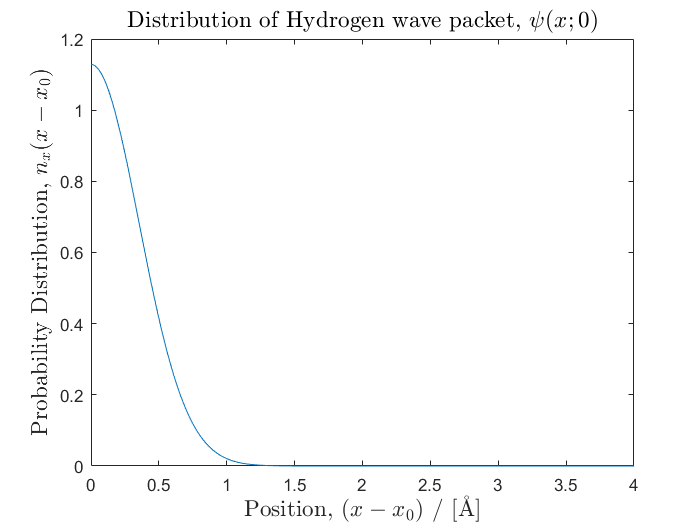
\includegraphics[width=\textwidth]{graphics/task1/position_prob.png}
		\caption{}
		\label{fig:1_a}
    \end{subfigure}
    \begin{subfigure}[b]{0.8\textwidth}
        \centering
        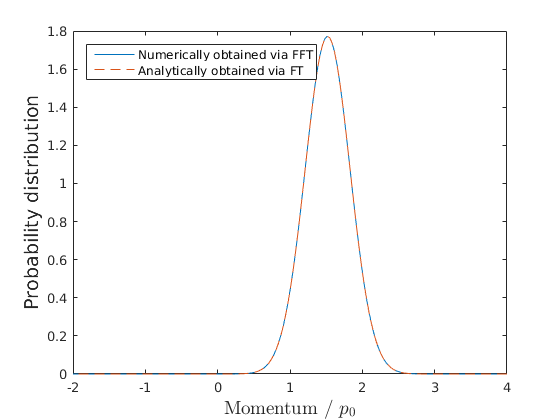
\includegraphics[width=\textwidth]{graphics/task1/momentum_prob.png}
        \caption{}
		\label{fig:1_b}
    \end{subfigure}
    \caption{\textit{(a):} The positive half of the wave packet in space. Given that it is a Gaussian distribution with zero mean, it is symmetrical around the y-axis. \textit{(b):} The wave packet in momentum space. The blue graph is the result obtained from numerically doing FFT on the initial wave packet. The red dashed graph is the analytical solution. Due to their similarity, the two graphs are difficult to distinguish from each other.}
    \label{fig:1}
\end{figure}


\section*{Problem 2}

\begin{figure}[H]
\centering
\begin{subfigure}[t]{0.7\textwidth}
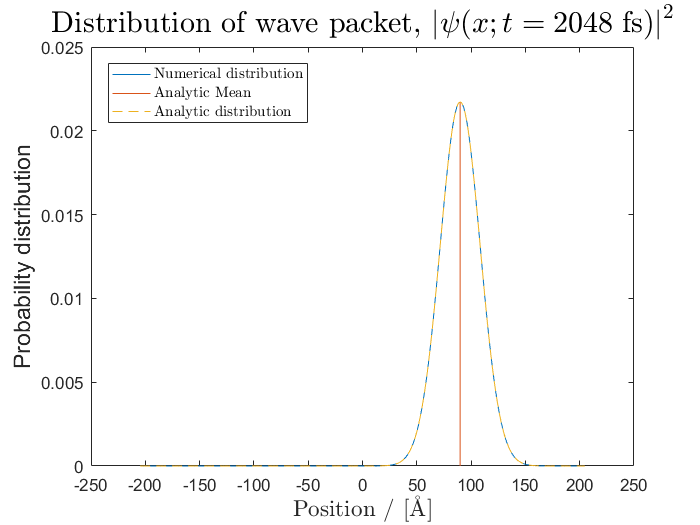
\includegraphics[width=\textwidth]{graphics/task2/position.png}
\caption{}
\label{fig:2_a}
\end{subfigure}

\begin{subfigure}[t]{0.7\textwidth}
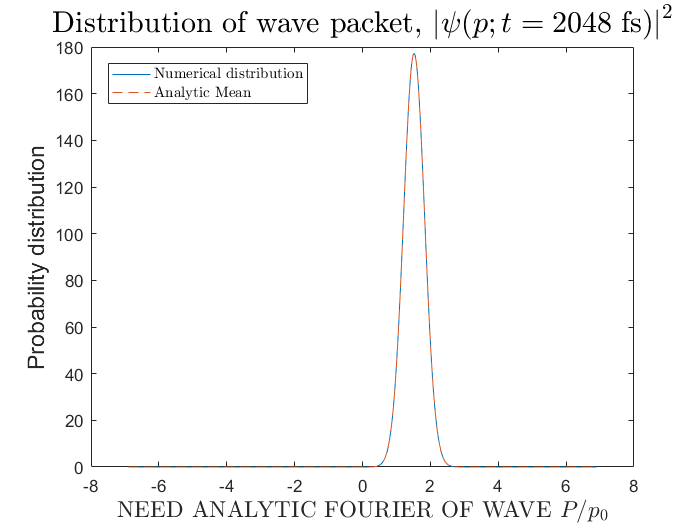
\includegraphics[width=\textwidth]{graphics/task2/momentum.png}
\caption{}
\label{fig:2_b}
\end{subfigure}

\begin{subfigure}[t]{0.7\textwidth}
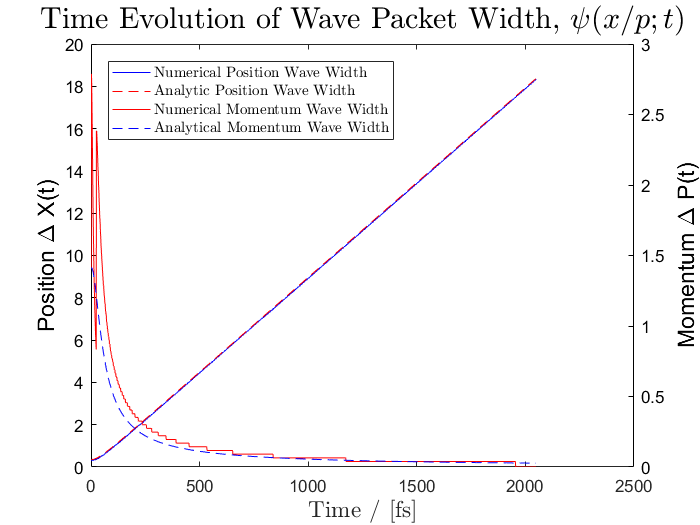
\includegraphics[width=\textwidth]{graphics/task2/width_evolution.png}
\caption{}
\label{fig:2_c}
\end{subfigure}

\caption{The distribution of the wave packets for position/momentum \textit{(a)}/\textit{(b)}, at time $\unit[2048]{fs}$. In \textit{(c)} the numerical time evolution of the width of the wave packets for both the position and momentum are compared with the analytical values.}
\label{fig:2}
\end{figure}

In the second task we simulated the movement of the same atom, moving in free space, using the split-operator FFT method and comparing the numerical result to analytical results.

The split-operator method is used the way described in the Introduction. Running the Matlab shows the actual time evolution, however the probability distribution for a given time in both the position and momentum domain can be found in Figure~\ref{fig:2}.

Figure~\ref{fig:2_c} also shows the time evolution of the width of the gaussian for both domains. As we can see, the width in the position domain increases as $y = x$ and $y = 1/x$ in the momentum domain, which is the expected behaviour. We also note that the numerical results align with the analytical ones very well.

The theoretical wave packet in the position domain is given by the expression
\begin{equation}
\psi(x,t) = \left[
\pi^{1/2}\left(
d+\frac{i\hbar t}{md}
\right)
\right]^{-1/2}
\exp\left[
\frac{-\left[x-\left(p_0/m\right)t\right]^2}{2d^2(1+iht/md^2)}
\right]
\exp\left[
\frac{ip_0}{\hbar}\left(x-\frac{p_0t}{2m}\right)
\right],
\end{equation}
yielding the wave packet,
\begin{equation}
\psi(p,t) = \frac{\sqrt{2} \pi^{1/4} \exp \left(-\frac{d^2 (\text{p0}-p \hbar )^2}{2 \hbar ^2}-\frac{i p^2 t \hbar }{2 m}\right)}{\sqrt{\frac{m}{d^2 m+i t \hbar }} \sqrt{d+\frac{i t \hbar }{d m}}},
\end{equation}
in the momentum domain.

The theoretical width of the packet grows according to,

\begin{equation}
\Delta X(t) =\frac{d}{2^{1/2}}\left(1+\frac{\hbar^2 t^2}{m^2 d^4}\right)^{1/2}
\end{equation}

and since the Gaussian wave packets fulfills the lower bound of the Heisenberg's uncertainty relation,

\begin{equation}
\Delta X \Delta P = \hbar/2
\end{equation}

which gives the expression for the uncertainty of the momentum as well\cite{Shankar:1994}.

which 



\section*{Problem 3}

\begin{figure}[H]

\centering
\begin{subfigure}[t]{0.47\textwidth}
	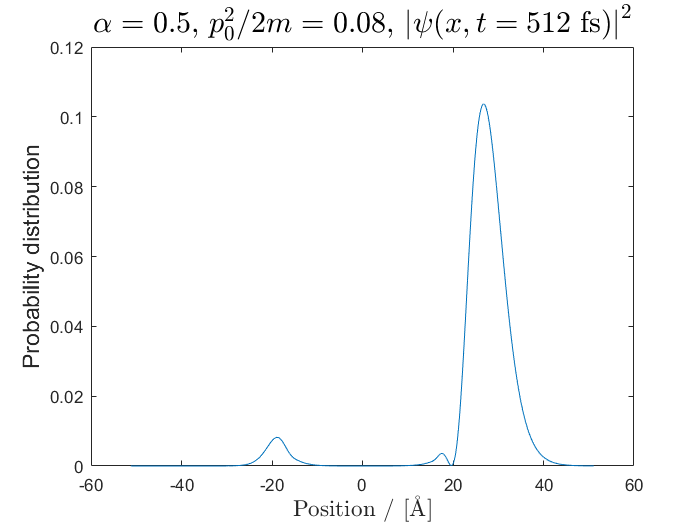
\includegraphics[width=\textwidth]{graphics/task3/a1e1.png}
	\caption{}
	\label{fig:3_a}
\end{subfigure}
\begin{subfigure}[t]{0.47\textwidth}
	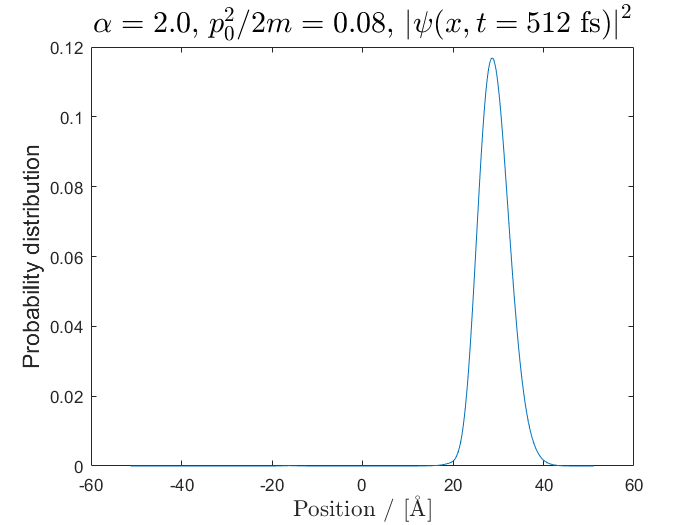
\includegraphics[width=\textwidth]{graphics/task3/a2e1.png}
	\caption{}
	\label{fig:3_b}
\end{subfigure}

\begin{subfigure}[t]{0.47\textwidth}
	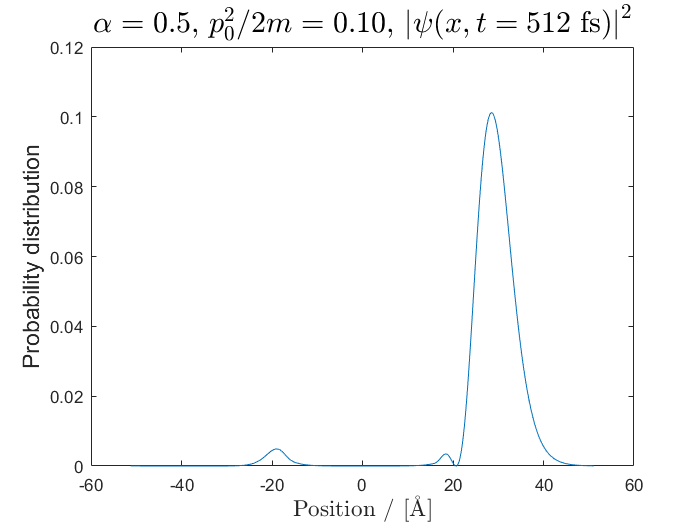
\includegraphics[width=\textwidth]{graphics/task3/a1e2.png}
	\caption{}
	\label{fig:3_c}
\end{subfigure}
\begin{subfigure}[t]{0.47\textwidth}
	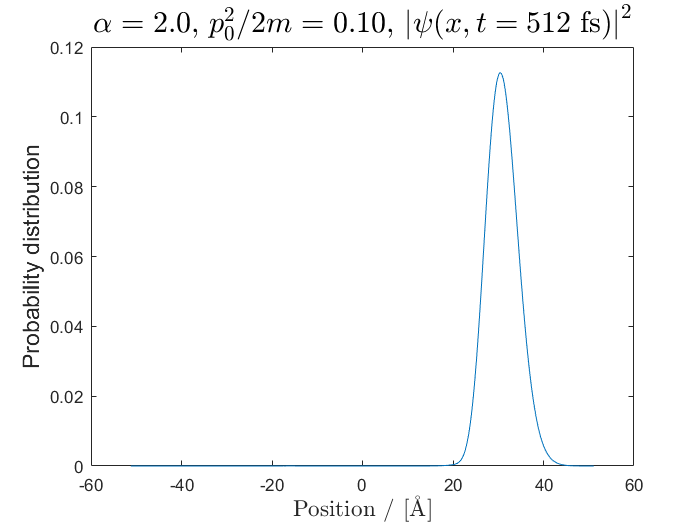
\includegraphics[width=\textwidth]{graphics/task3/a2e2.png}
	\caption{}
	\label{fig:3_d}
\end{subfigure}

\begin{subfigure}[t]{0.47\textwidth}
	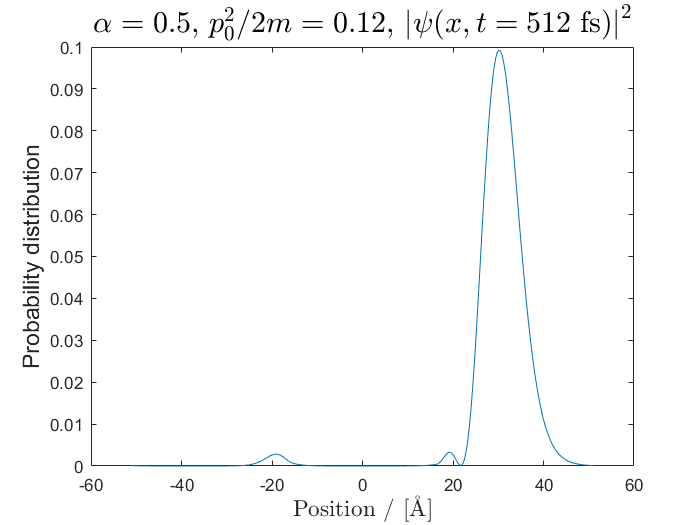
\includegraphics[width=\textwidth]{graphics/task3/a1e3.png}
	\caption{}
	\label{fig:3_e}
\end{subfigure}
\begin{subfigure}[t]{0.47\textwidth}
	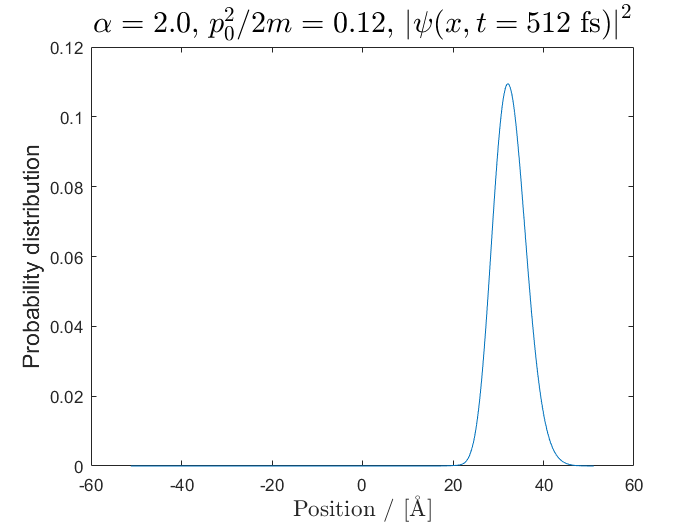
\includegraphics[width=\textwidth]{graphics/task3/a2e3.png}
	\caption{}
	\label{fig:3_f}
\end{subfigure}

\caption{The scattered probability densities for the 6 different cases. In the left column we have $\alpha = 0.5$ and in the right $\alpha=2.0$. For the different rows we have $p_0^2/2m=0.08, 0.10, 0.12$ top down. }
\label{fig:3}
\end{figure}

\begin{table}[H]
	\centering
	\caption{Table of the probabilities of scattering ($n_<$) and transmission ($n_>$) through the Eckhart barrier. All entries have been rounded to four significant numbers, except for $\alpha = 2.0$, $p_0^2/2m = 0.12$, resulting in that they don't necessarily sum to unity.}
	\begin{tabular}{c|cc|cc}
					& \multicolumn{4}{c}{\textbf{Probability}} \\
					& \multicolumn{2}{c|}{$\alpha = 0.5$} & \multicolumn{2}{c}{$\alpha = 2.0$} \\
		$p_0^2/2m$	& $n_<(t)$	& $n_>(t)$	& $n_<(t)$	& $n_>(t)$	\\ \hline
		0.08 eV		& 0.0517	& 0.9483	& $4.256 \cdot 10^{-4}$	& 0.9996	\\
		0.10 eV		& 0.0304	& 0.9696	& $9.946 \cdot 10^{-5}$	& 0.9999	\\
		0.12 eV		& 0.0177	& 0.9823	& $2.7531 \cdot 10^{-5}$ & 0.99998
	\end{tabular}
	\label{tab:3}
\end{table}

In the third task we scatter the same particle against a one-dimensional Eckhart barrier so we do not have a free particle, but we have a potential described by,
\begin{equation}
V(x) = V_0 \cosh^{-2} (x/\alpha),
\end{equation}

with $V_0 = \unit[0.1]{eV}$.

Three cases are studied: $p_0^2/2m$ = 0.08 eV, 0.10 eV and 0.12 eV. The results are shown in Figure~\ref{fig:3}. We see that the particle scatters only significantly for $\alpha = 0.5$.





\bibliography{references}
\bibliographystyle{plain}

\appendix
\section{Source code}

\subsection{\texttt{main1.m}}
\lstinputlisting[language=matlab, numbers=left]{../code/main1.m}

\subsection{\texttt{main2.m}}
\lstinputlisting[language=matlab, numbers=left]{../code/main2.m}

\subsection{\texttt{main3.m}}
\lstinputlisting[language=matlab, numbers=left]{../code/main3.m}

%\subsection{\texttt{main4.m}}
%\lstinputlisting[language=matlab, numbers=left]{../code/main4.m}

\end{document}